\documentclass[journal]{IEEEtran}

\usepackage{graphicx}
\usepackage{float}
\usepackage{amsmath}
\usepackage{algorithm}
\usepackage[noend]{algpseudocode}
\usepackage{mathtools}
\DeclarePairedDelimiter\floor{\lfloor}{\rfloor}

\renewcommand\refname{Daftar Pustaka}
\renewcommand{\figurename}{Gambar}
\renewcommand{\tablename}{Tabel}

\begin{document}
	
\title{Kompresi Data pada Laporan Cuaca Menggunakan Metode \textit{Huffman Coding}}

\author{
	IF 38-01\\
	\vspace{1mm}
	Aliya Nur Rezkita\hspace{1.05cm} 1301144161\\
	Febby Febriansyah\hspace{1cm} 1301140371\\	
	Rizkiyana Prima Putra\hspace{0.4cm} 1301140181\\
	Tari Lestari\hspace{2.15cm} 1301144281\\
	Fakultas Informatika, Telkom University, Bandung
}

\markboth{Tugas Besar Dasar Pemodelan dan Simulasi IF 38-01}%
{Shell}

\maketitle

\begin{abstract}
	ini abstrak ... ...
\end{abstract}

\begin{IEEEkeywords}
Data Compression, Huffman Coding, Weather Report, Probability.
\end{IEEEkeywords}


\section{Pendahuluan}
\hspace*{0.7cm}Banyak kegiatan atau aktifitas manusia yang banyak bergantung pada faktor cuaca. Faktor cuaca ini terkadang memiliki pengaruh yang sangat besar bagi keberlangsungan kegiatan yang dilakukan. Peran seorang prakiawan cuaca sangat dibutuhkan, mengingat cuaca adalah kondisi udara yang berlangsung dalam jangka waktu yang singkat. Maka, proses prakiraan cuaca jangka pendek harus dilakukan secara cepat dan seakurat mungkin. Kondisi cuaca di suatu tempat ditentukan oleh sejumlah faktor diantaranya temperatur udara, kelembaban udara, arah angin, kecepatan angin dan sebagainya. Dengan melihat faktor-faktor ini, seorang prakiawan cuaca dapat memprediksikan kondisi cuaca yang akan berlangsung pada keesokan harinya.\\
\hspace*{1cm}Berbagai metode dilakukan untuk memperoleh hasil informasi cuaca yang akurat, salah satunya menggunakan pendekatan model cuaca numerik. Perkembangan model cuaca numerik seiring dengan perkembangan kemampuan komputasi dan penambahan jaringan pengamatan telah mencapai akurasi prediksinya yang baik dan sudah banyak digunakan dalam membuat prakiraan cuaca oleh pusat layanan cuaca di banyak negara. Pola cuaca yang berbeda antar wilayah, mengharuskan dilakukan pengujian model cuaca numerik seperti pemilihan skema parameterisasi, syarat awal, waktu “spin-up” agar mampu menghasilkan prediksi yang terbaik. (Indra Gustari, dkk. Jurnal Meteorologi dan Geofisika Vol. 13 No. 2: 119-130. 2012).\\
\hspace*{1cm}Metode cuaca numerik yang banyak digunakan adalah Numerical Weather Prediction (NWP). NWP menggunakan representasi keadaan atmosfer secara numerik baik global maupun regional untuk memprediksi kondisi atau keadaan atmosfer yang akan datang dengan menggunakan berbagai persamaan-persamaan yang berlaku di atmosfer (Pielke R.A, 2002, Mesoscale Meteorological Modeling, Academic Press, pp 48–49).\\
\hspace*{1cm}NWP adalah sekumpulan kode komputer yang mempresentasikan secara numerik persamaan-persamaan atmosfer, digunakan untuk memprediksi kondisi atau status atmosfer yang akan datang dengan menggunakan kemampuan komputer yang tinggi. Prediksi atau ramalan cuaca dirumuskan dengan menyelesaikan persamaan pergerakan atmosfir. Persamaan–persamaan tersebut meliputi persamaan non-linier time-dependent differential partial angin, temperatur, kelembaban dan tekanan (Lynch, P. 2006).\\
\hspace*{1cm}Metode NWP melibatkan perhitungan parameter cuaca yang cukup banyak, umumnya prakiraan cuaca yang menggunakan metode ini mempunyai keluaran (file output) yang cukup besar. Besar kecilnya hasil keluaran ditentukan oleh beberapa faktor, antara lain: luas daerah yang diprediksi, panjang prediksi, resolusi spasial yang digunakan, dan parameter cuaca yang dihasilkan. (Wido Hanggoro, Iis Widya Harmoko, Setyawan Widyarto, 2012)\\
\hspace*{1cm}Untuk Kota Bandung yang mempunyai wilayah yang cukup luas, penggunaan metode NWP akan memberikan permasalahan yang cukup signifikan dalam hal distribusi dan penyimpanan data-data prediksi cuaca. Ditambah lagi penggunaan dynamical downscaling (perolehan informasi spasial cuaca yang lebih detil/resolusi tinggi) untuk peningkatan akurasi prakiraan yang akan semakin memperbesar ukuran file output. Oleh karena itu, dibutuhkan suatu proses pengubahan sekumpulan data menjadi suatu bentuk kode untuk menghemat kebutuhan tempat penyimpanan dan waktu untuk transmisi data.\\
\hspace*{1cm}Dalam makalah ini, pengubahan bentuk data menjadi kode akan menggunakan Algoritma Huffman yaitu algoritma yang tiap karakter (simbol) dikodekan hanya dengan rangkaian beberapa bit, dimana karakter yang sering muncul dikodekan dengan rangkaian bit yang pendek dan karakter yang jarang muncul dikodekan dengan rangkaian bit yang lebih panjang sehingga akan mempermudah untuk menyelesaikan suatu masalah perkiraan cuaca.

\section{Metode Penelitian}
\hspace*{0.7cm}Tahapan penelitian yang akan dilakukan dalam makalah ini adalah menggunakan algoritma Huffman untuk pengubahan sekumpulan data menjadi suatu bentuk kode agar menghemat kebutuhan tempat penyimpanan dan waktu transmisi data.\\
\\
\textbf{\textit{Algoritma Huffman}}\\
\hspace*{0.7cm}Permasalahan dalam makalah ini akan diselesaikan dengan pengkodean huffman dari string $4^n$ dengan panjang $n$ pada alfabet {S, C, R, F}, dimana dengan probabilitas sebuah string dengan $f_S$ S's, $f_C$ C's, $f_R$ R's dan $f_F$ F's adalah ${P^S}_{sunny}$ . ${P^fc}_{cloudy}$ . ${P^R}_{rainy}$ . ${P^F}_{foggy}$ , namun $4^n$ sangat besar sehingga tidak dapat mensimulasikan prosedur pengkodean huffman secara sederhana. Namun, karena struktur produk dari distribusi, akan ada banyak node dalam pengkodean huffman yang memiliki probabilitas yang sama, jadi kita dapat mengelompokkannya dan tetap menghitungnya.\vspace*{1mm}
\hspace*{1cm}Awalnya ada $\binom{n}{f_S,f_C,f_R,f_F} = \frac{n!}{f_s! f_c! f_R! f_F!}$ node\vspace*{1mm} dengan probabilitas ${P^S}_{sunny} , {P^fc}_{cloudy} , {P^R}_{rainy} , {P^F}_{foggy}$ (untuk setiap kombinasi nilai non-negatif $f_S, f_C, f_R, f_F$ penjumlahan sampai $n$). Sekarang kita lanjutkan dengan huffman encoding: pilih node probabilitas terkecil, misal probabilitas ini adalah $p$. Jika ada $K$ node dengan probabilitas ini, maka akan menimbulkan $\floor*{K / 2}$ node dari probabilitas $2p$, dan jika $K$ adalah bilangan ganjil maka satu node dari probabilitas $p$ yang tersisa akan di cocokan dengan salah satu node dengan nilai probabilitas terkecil kedua.\\
\\
Langkah-langkah pembentukan pohon Huffman adalah sebagai berikut :
\begin{enumerate}
	\item Baca semua karakter di dalam teks untuk menghitung frekuensi kemunculan setiap karakter. Setiap karakter penyusun teks dinyatakan sebagai pohon bersimpul tunggal. Setiap simpul di-assign dengan frekuensi kemunculan karakter tersebut.
	\item Terapkan strategi algoritma sebagai berikut, gabungkan dua buah pohon yang mempunyai frekuensi terkecil pada sebuah akar. Setelah digabungkan, akar tersebut akan mempunyai frekuensi yang merupakan jumlah dua buah pohon-pohon penyusunnya.
	\item Ulangi langkah 2 sampai hanya tersisa satu buah pohon Huffman. Agar pemilihan dua pohon yang akan digabungkan berlangsung cepat, maka semua pohon yang ada selalu terurut menaik berdasarkan frekuensi.
\end{enumerate}
Sebagai contoh, dalam kode ASCII string 7 huruf “ABACCDA” membutuhkan representasi 7 x 8 bit = 56 bit (7 byte), dengan rincian sebagai berikut:
\begin{center}
	A = 01000001\\
	B = 01000010\\
	A = 01000001\\
	C = 01000011\\
	C = 01000011\\
	D = 01000100\\
	A = 01000001\\
\end{center}
Pada string tersebut, frekuensi kemunculan A = 3, B = 1, C=2, dan D = 1, sehingga proses pembentukan pohon Huffman-nya adalah seperti yang ditampilkan pada gambar berikut:
\begin{figure}
	\centering
	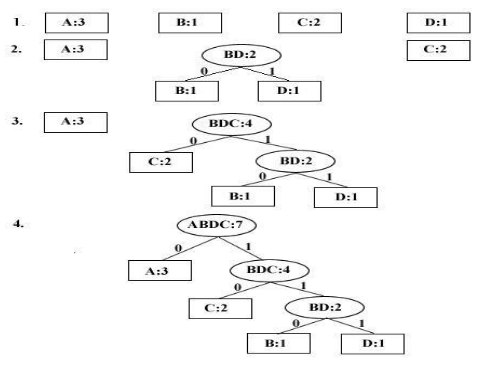
\includegraphics[width=\linewidth]{Capture.png}
	\caption{Tree Algoritma Huffman}
	\label{fig:tree}
\end{figure}
\section{Hasil Penelitian}
hasilnya.......


\section{Kesimpulan}
Kesimpulan ... ... ...

\begin{thebibliography}{5}

\bibitem{zhu}
Xuezhi Zhu, Wenjian Lou, and Tao Zhu,
\textit{An Improved Genetic Algorithm for Dynamic Shortest Path Problems},
School of Computer Science and Technology, University of Science and Technology of China, Hefei 230027, Anhui, China, 2014.

\bibitem{hardi}
Richki Hardi,
\textit{Genetic Algorithm in Solving the TSP on These Mineral Water},
Department of Informatics Engineering, Sekolah Tinggi Teknologi Bontang, Indonesia, 2015.

\bibitem{goldberg}
Goldberg, D. E.,
\textit{Genetic Algorithms in Search, Optimization, and Machine Learning},
Addison-Wesley, England, 1989.

\bibitem{holland}
J. H. Holland,
\textit{Adaptation in Natural and Artificial System},
The University of Michigan Press, 1975.

\bibitem{poddar}
Rajarshi Poddar, Subarno Banerjee, and Parag Kumar Guha Thakurta,
\textit{Shortest Path Routing for Co-ordinate Based Mobile Networks: A Genetic Algorithm Approach},
Dept. of Computer Science and Engineering, National Institute of Technology, Durgapur, India, 2012.

\bibitem{lau}
H. C. W. Lau, T. M. Chan, and W. T. Tsui,
\textit{Fuzzy Logic Guided Genetic Algorithms for the Location Assignment of Items},
IEEE Congress on Evolutionary Computation (CEC 2007), 2007.

\end{thebibliography}

\end{document}


